\documentclass[zavrsnirad]{fer}
% Dodaj opciju upload za generiranje konačne verzije koja se učitava na FERWeb
% Add the option upload to generate the final version which is uploaded to FERWeb

\usepackage{blindtext}
\usepackage{float}
\usepackage{adjustbox}
\usepackage{listings}


% Define custom colors for syntax highlighting
\definecolor{mygreen}{rgb}{0,0.6,0}
\definecolor{mygray}{rgb}{0.5,0.5,0.5}
\definecolor{mymauve}{rgb}{0.58,0,0.82}

% Define the style for listings
\lstdefinestyle{mystyle}{
	backgroundcolor=\color{white},   % choose the background color
	basicstyle=\linespread{1.2}\ttfamily\footnotesize, % size of fonts used for the code
	breakatwhitespace=false,         % sets if automatic breaks should only happen at whitespace
	breaklines=true,                 % sets automatic line breaking
	captionpos=b,                    % sets the caption-position to bottom
	commentstyle=\color{mygreen},    % comment style
	escapeinside={\%*}{*)},          % if you want to add LaTeX within your code
	keywordstyle=\color{blue},       % keyword style
	stringstyle=\color{mymauve},     % string literal style
	numbers=left,                    % where to put the line-numbers; possible values are (none, left, right)
	numberstyle=\tiny\color{mygray}, % the style that is used for the line-numbers
	stepnumber=1,                    % the step between two line-numbers. If it's 1, each line will be numbered
	numbersep=5pt,                   % how far the line-numbers are from the code
	showspaces=false,                % show spaces adding particular underscores; it overrides 'showstringspaces'
	showstringspaces=false,          % underline spaces within strings only
	showtabs=false,                  % show tabs within strings adding particular underscores
	tabsize=2,                       % sets default tabsize to 2 spaces
}
% Apply the style to the listings package
\lstset{style=mystyle}



%\begin{lstlisting}[language=Python]
%	import math
%	
%	def example_function(x):
%	# This is a comment
%	if x > 0:
%	return math.sqrt(x)
%	else:
%	return "Input must be positive"
%	
%	print(example_function(9))
%	print(example_function(-1))
%\end{lstlisting}
%
%\section{C++ Example}
%Here is an example of C++ code with syntax highlighting:
%
%\begin{lstlisting}[language=C++]
%	#include <iostream>
%	#include <cmath>
%	
%	int main() {
%		int x = 9;
%		// This is a comment
%		if (x > 0) {
%			std::cout << sqrt(x) << std::endl;
%		} else {
%			std::cout << "Input must be positive" << std::endl;
%		}
%		return 0;
%	}
%\end{lstlisting}



%--- PODACI O RADU / THESIS INFORMATION ----------------------------------------

% Naslov na engleskom jeziku / Title in English
\title{Visualization of public transport traffic in real time using the format
	GTFS}

% Naslov na hrvatskom jeziku / Title in Croatian
\naslov{Vizualizacija prometa javnog prijevoza u stvarnom vremenu uporabom formata
	GTFS}

% Broj rada / Thesis number
\brojrada{1246}

% Autor / Author
\author{Luka Miličević}

% Mentor 
\mentor{izv. prof. dr. sc.\@ Ivana Bosnić}

% Datum rada na engleskom jeziku / Date in English
\date{June, 2024}

% Datum rada na hrvatskom jeziku / Date in Croatian
\datum{lipanj, 2024.}

%-------------------------------------------------------------------------------


\begin{document}

% Naslovnica se automatski generira / Titlepage is automatically generated
\maketitle


%--- ZADATAK / THESIS ASSIGNMENT -----------------------------------------------

% Zadatak se ubacuje iz vanjske datoteke / Thesis assignment is included from external file
% Upiši ime PDF datoteke preuzete s FERWeb-a / Enter the filename of the PDF downloaded from FERWeb
\zadatak{figures/hr_0036543289_73.pdf}


%--- ZAHVALE / ACKNOWLEDGMENT --------------------------------------------------

\begin{zahvale}
  % Ovdje upišite zahvale / Write in the acknowledgment
  Hvala na kavi...
\end{zahvale}


% Odovud započinje numeriranje stranica / Page numbering starts from here
\mainmatter


% Sadržaj se automatski generira / Table of contents is automatically generated
\tableofcontents


%--- UVOD / INTRODUCTION -------------------------------------------------------
\chapter{Uvod}
\label{pog:uvod}

U velikim urbanim gradovima poput Zagreba, javni gradski prijevoz predstavlja neizostavan dio svakodnevnog života. On je temeljni stup mobilnosti, pružajući vitalnu infrastrukturu za povezivanje građana i omogućujući lakše i efikasnije kretanje unutar grada. Velika većina građana svakodnevno koristi javni prijevoz te s obzirom na važnost vremena u užurbanom ritmu gradskog života, dobra organizacija i planiranje putovanja su ključni, jer svi bi htjeli 15 minuta koje potroše na čekanju prijevoza iskoristiti na drukčiji način. Upravo s tim ciljem, ideja završnog rada je stvoriti web aplikaciju, koja pruža stvarno praćenje tramvaja u realnom vremenu, olakšavajući korisnicima efikasno planiranje svojih putovanja, osiguravajući im precizne informacije o dolasku tramvaja i informacijama o pojedinim gradskim linijama prijevoza. Kroz ovaj zadatak, istražit ćemo tehničke izazove s kojima se susrećemo u razvoju takve web aplikacije. Dublje ćemo istražiti ključne elemente koji oblikuju temelje naše aplikacije poput analize API-ja pruženog od strane Zagrebačkog Električnog Tramvaja, proučavanje otvorenih standarda GTFS i GTFS realtime, te detaljniju analizu strukture web-aplikacije, od baze podataka PostgreSQL, poslužiteljskog dijela ostvarenog s node.js i Express.js, do klijentskog dijela implementiranog s React.js i bibliotekama poput Leaflet.js




%\begin{figure}[htb]
%  \centering
%  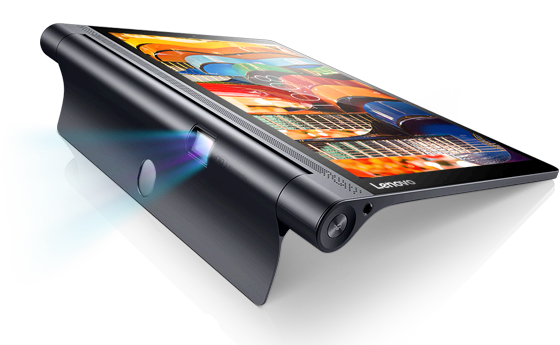
\includegraphics[width=0.38\linewidth]{Figures/lenovo_yoga_tab3_pro_front.png} 
%  \caption{Moja prva slika}
%  \label{slk:prvaslika}
%\end{figure}

%Referenciramo se na sliku \ref{slk:prvaslika} u sredini rečenice, zatim prije zareza %\ref{slk:prvaslika}, te zatim na kraju rečenice \ref{slk:prvaslika}.
%Upravo smo testirali radi li naredba \verb|\ref| ispravno u slučaju kada nakon nje slijedi točka.


%-------------------------------------------------------------------------------
\chapter{Glavni dio}
\label{pog:glavni_dio}

\section{Zagrebački Električni Tramvaj}

Zagrebački električni tramvaj, poznatiji kao ZET, je trgovačko društvo koje je u direktnom
vlasništvu Grada Zagreba, te ima ključnu ulogu u organizaciji javnog gradskog prijevoza u Zagrebu.
Posluje od 1910. godine i svakodnevno pruža prijevozne usluge za gotovo milijun ljudi pomoću
tramvaja, autobusa, uspinjače i specijalnih prijevoza \cite{ZET}.
Nedavno je ZET otvorio svoje podatke javnosti pod Otvorenom dozvolom Republike Hrvatske. Ovi podaci obuhvaćaju GTFS static i GTFS realtime podatke \ref{sec:GTFS}, koji su trenutno parcijalno implementirani te su dostupni na službenoj stranici ZET-a \cite{ZET-GTFS}.
Ti podaci će biti temelj aplikacije i kroz njih ćemo detaljnije proći u narednim poglavljima \ref{sec:zet-gtfs}

\subsubsection{Slične aplikacije - ZET info}
Jedna popularna aplikacija koja koristi iste ZET-ove podatke je ZET info \cite{ZET-info}. Koja primarno koristi GTFS static podatke za prikaz rasporeda tramvaja ZET-a. Ona nije službena ZET-ova aplikacija te dostupna je preko Apple App Store-a i Google play-a. Vrlo je zgodna za imati pri ruci za pregledavanje rasporeda vožnji, ali bi aplikacijom ovog završnog rada htjeli ostvariti i upotrebu stvarnih (realtime) podatatak za tramvaje.


\begin{figure}[htb]
	\centering
	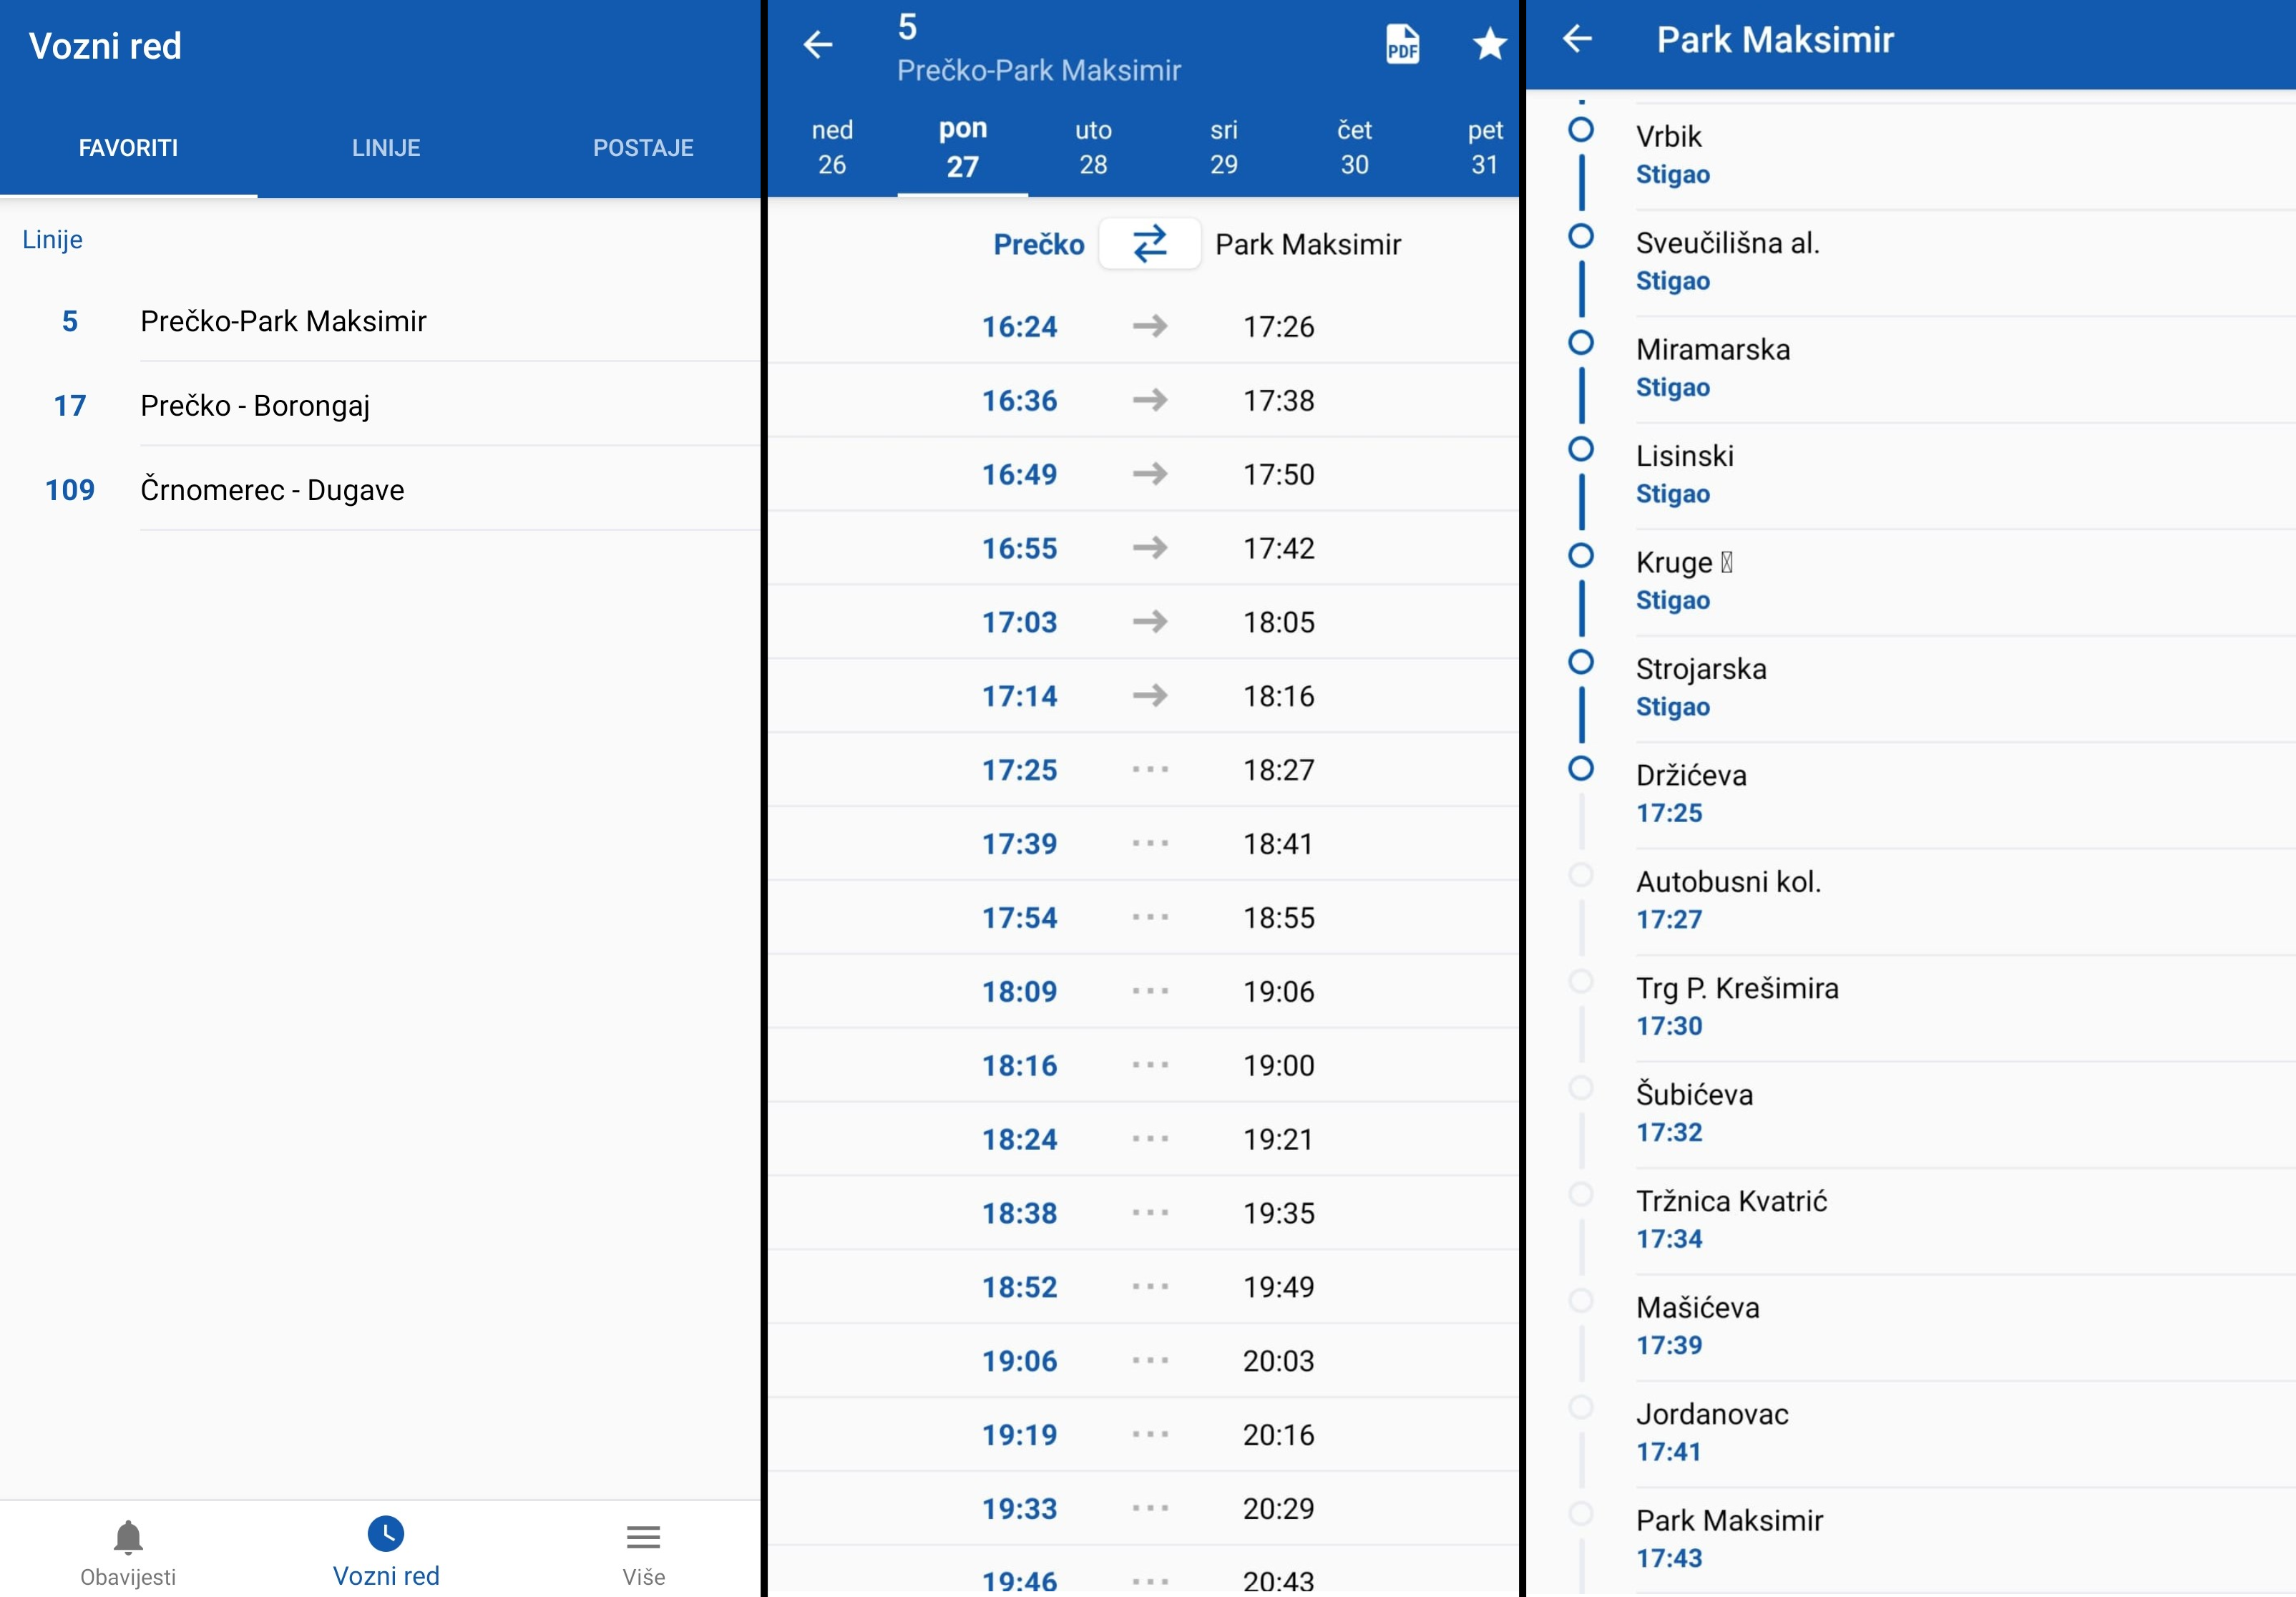
\includegraphics[width=0.85\linewidth]{Figures/zetinfo.png} 
	\caption{ZET info}
	\label{slk:zet-info}
\end{figure}

\newpage
\section[GTFS]{General Transit Feed Specification}
\label{sec:GTFS}

General Transit Feed Specification, kraće GTFS je otvoreni standardizirani format za rasporede
javnog prijevoza i pripadajuće geografske informacije. Široko se koristi diljem svijeta te ga
podržavaju više od 10 tisuća agencija javnog prijevoza u preko 100 zemalja. Neke od platformi koje
koriste GTFS su Google Maps, Apple Maps, Moovit, OpenStreetMap i druge \cite{GTFS}. GTFS je započeo 2005. godine kao ideja za sporedni projekt Googleovog zaposlenika Chris Harrelsona te je danas \textit{De facto} standard industrije. GTFS se sastoji od dva glavna dijela GTFS schedule (static) i GTFS realtime.

Činjenica da je GTFS otvoreni standard omogućuje da agencije za prijevoz informacije učine dostupnima pomoću bilo kojeg od mnogih alata koji već podržavaju GTFS i korisnicima da preuzmu i obrađuju te informacije sa proizvoljnom aplikacijom koja podržava GTFS ili ako žele razviju svoje programe za to. Otvoreni standardi dovode do stvaranja podataka koji se mogu lako dijeliti i potiču daljnji razvitak.

Jedan zanimljiv primjer male aplikacije koja koristi GTFS podatke da prikaže područja na karti do kojih možete doći javnim prijevozom u određenom vremenu je otvoreni projekt Mapnificent koji je javno dostupan na Github-u \cite{Mapnificent}. Na slici \ref{slk:mapnificent-zagreb} je prikazano dokle je moguće doći javnim prijevozom od zgrade FER-a unutar 12 minuta. 

\begin{figure}[htb]
  \centering
  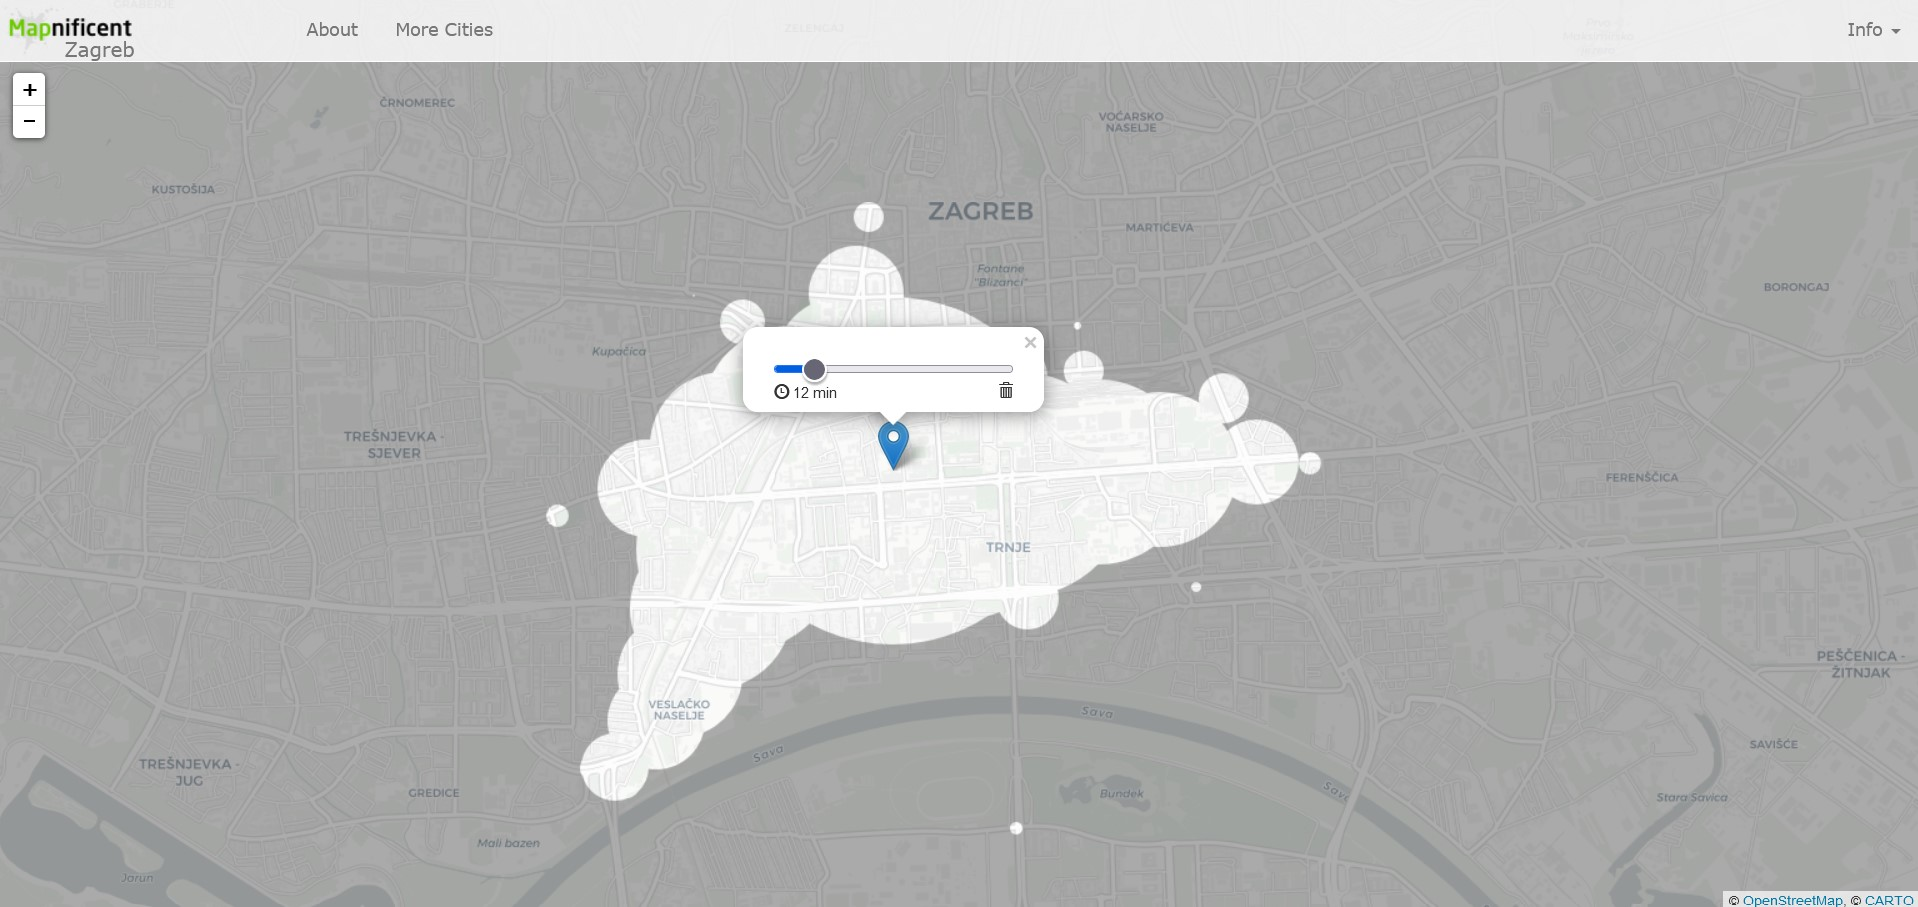
\includegraphics[width=0.9\linewidth]{Figures/mapnificent-zagreb.jpg} 
  \caption{Mapnificent Zagreb}
  \label{slk:mapnificent-zagreb}
\end{figure}

\subsection{GTFS static}

GTFS static ili GTFS schedule je kolekcija od barem 6 osnovnih, do 26 CSV (comma-separated
values) datoteka s ekstenzijom .txt zapakiranih unutar jedne komprimirane .zip datoteke. Te datoteke
sadrže informacije o rutama, rasporedima, stanicama, i ostalim raznim informacijama o prijevozu \cite{GTFS-schedule}. Sam format datoteka koji je CSV, pruža otvorenost i jednostavnost rukovanja jer mnogo programskim alata i jezika ima metode za efektivnu obradu CSV što čini implementaciju strojnog čitanja lakoćom. Važno za napomenuti da je način kodiranja datoteka imperativan, obavezuje se korištenje UTF-8 kodiranja (podržan je i UTF-8 BOM).


Na dijagramu \ref{slk:gtfs-model} prikazan je jedan primjer važeće strukture GTFS static modela kojeg prikladno prikazuju datoteke u ER (Entity–relationship) modelu. Zelenom bojom su označene neophodne datoteke, a plavom par dodatnih opcionalnih datoteka te za svaku od njih struktura i međusobne relacije. 

\begin{figure}[H]
	\centering
	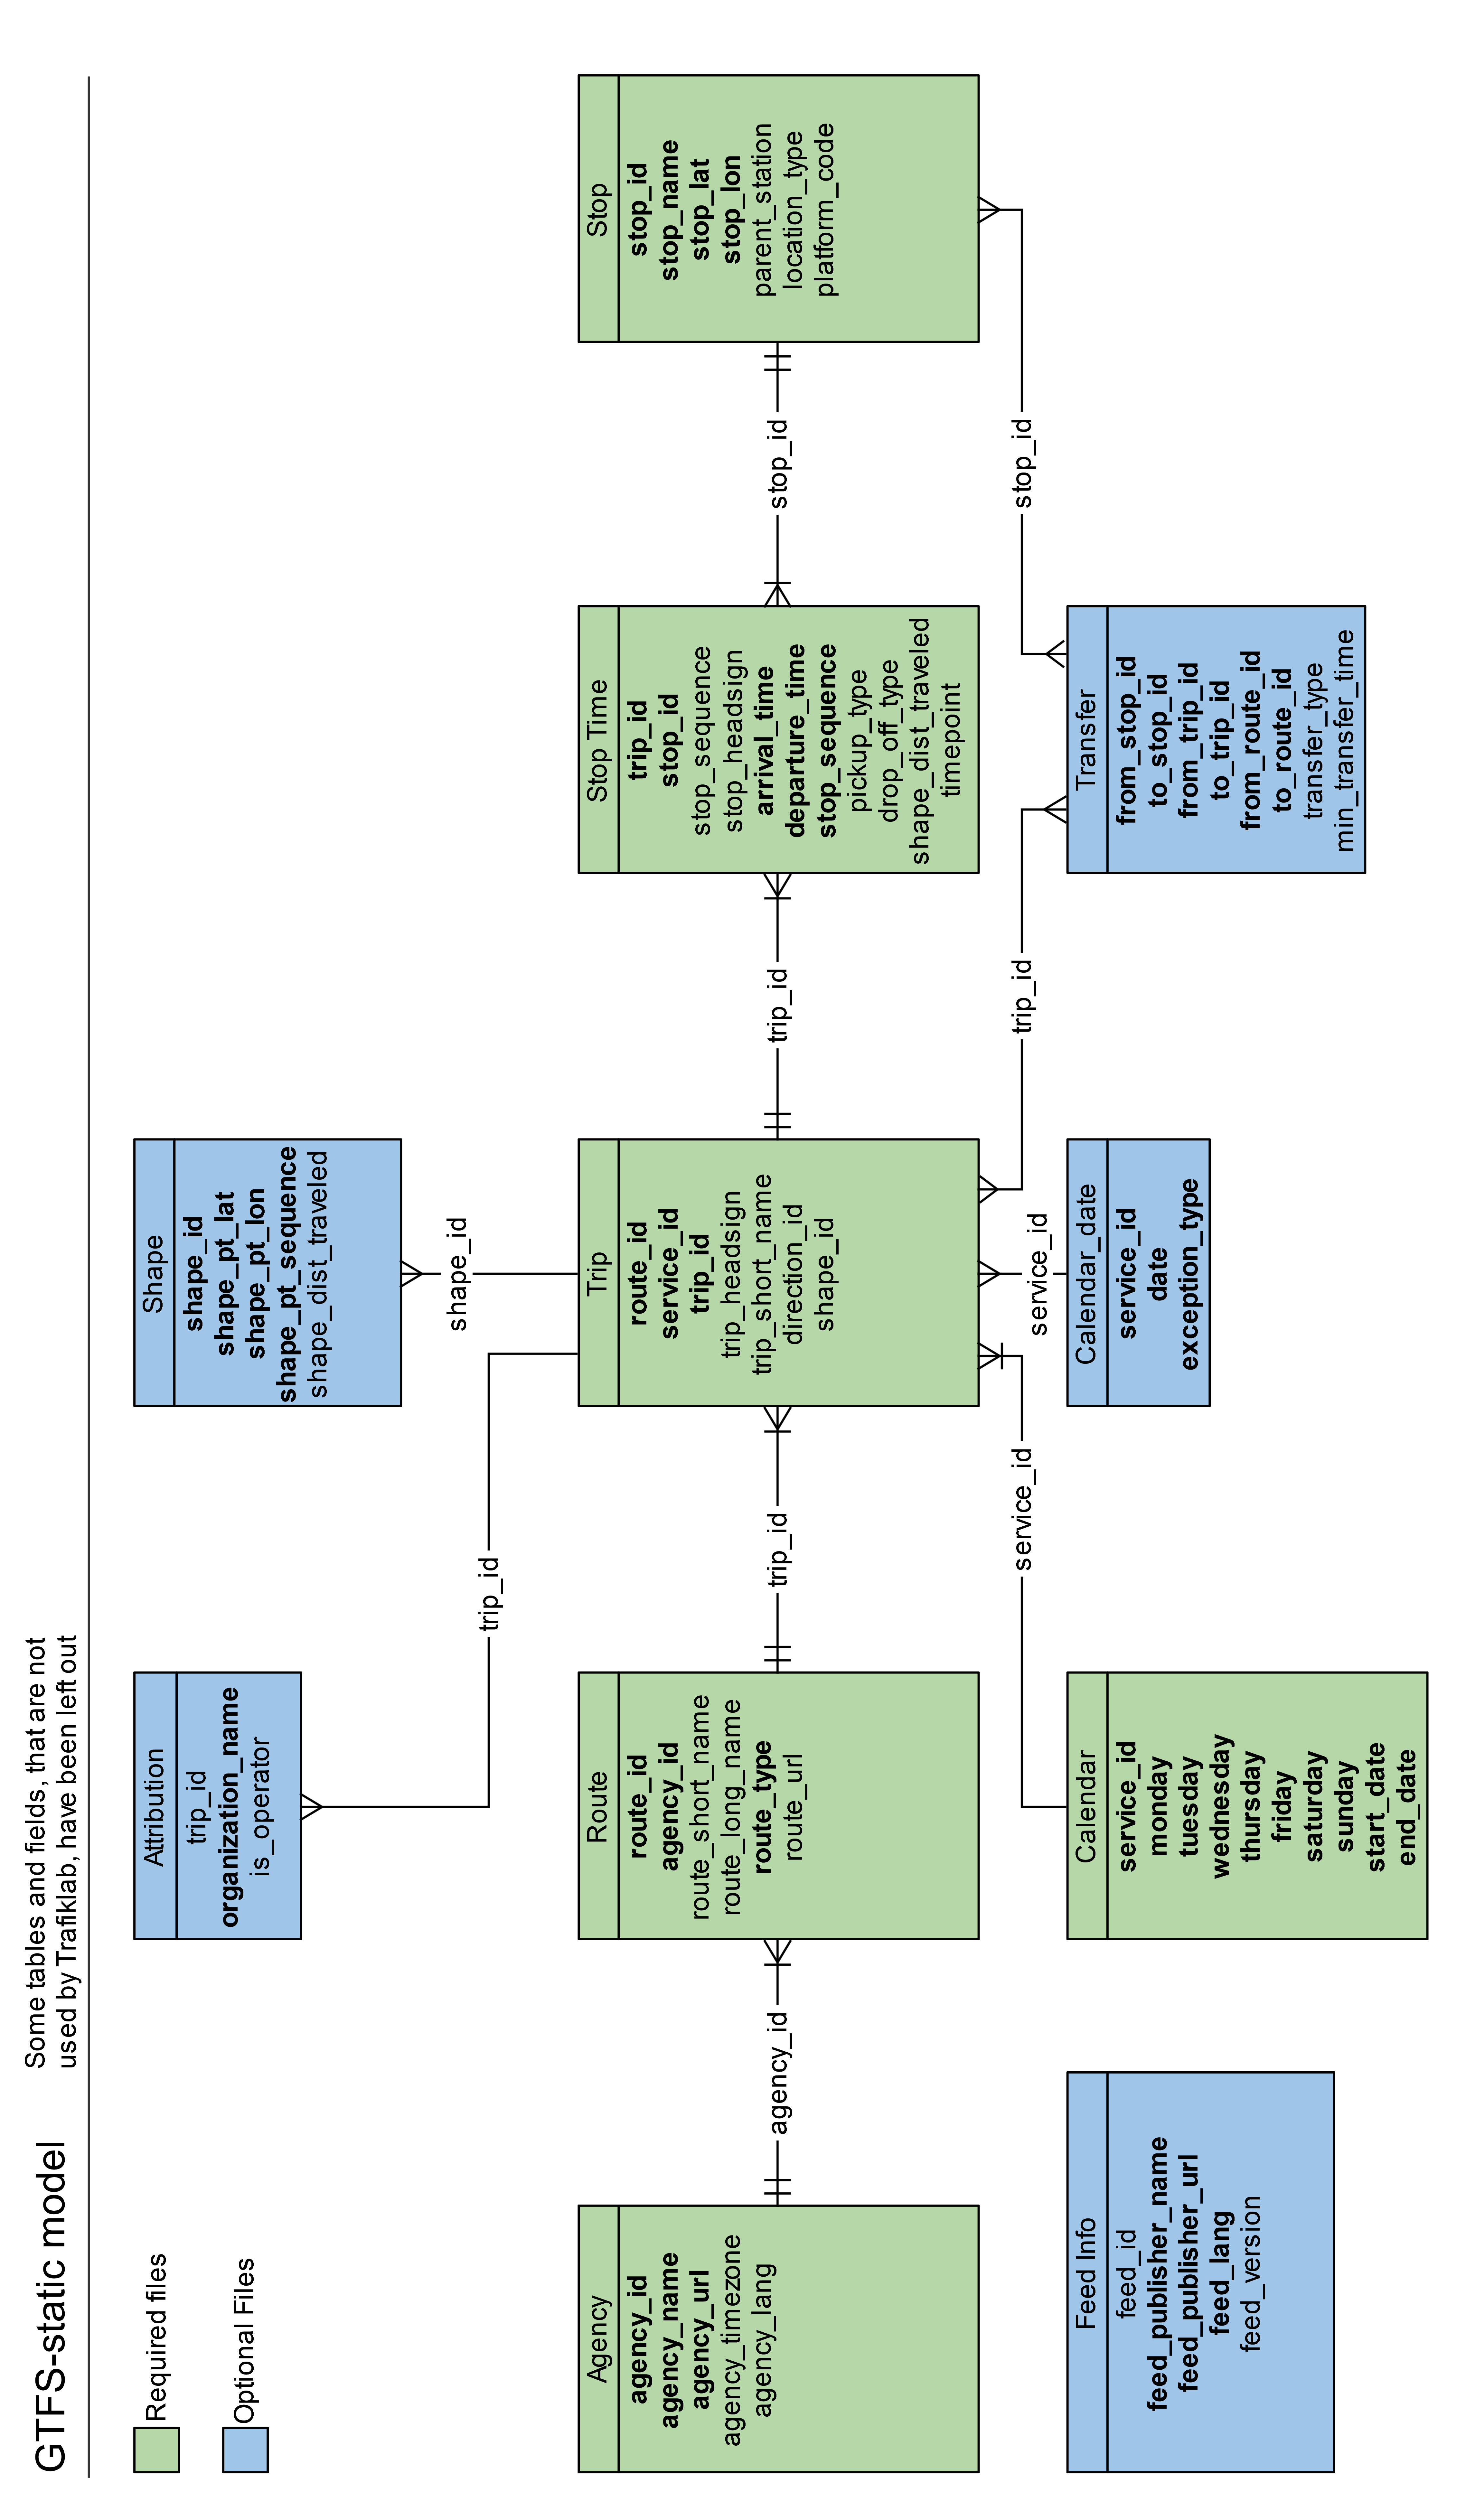
\includegraphics[width=\linewidth-30pt]{Figures/gtfs-model.png}
	\caption{GTFS-static model \cite{GTFS-schedule-model}}
	\label{slk:gtfs-model}
\end{figure}

\newpage

\subsubsection{Neophodne datoteke}
Moraju biti definirane da bi zadovoljili GTFS standard. One spojene zajedno pomoću pojedinih identifikatora čine cjelovitu sliku mreže javnog prijevoza
\begin{itemize}
	\item \textbf{Agency.txt} -
	Opće informacije o prijevoznoj agenciji, uključujući njezino ime, web stranicu, i vremensku zonu.
	\item \textbf{Routes.txt} -
	Definira različite linije javnog prijevoza. Svaka ruta obuhvaća informacije o identifikatorima ruta, tipovima vozila i drugim detaljima.
	\item \textbf{Trips.txt} -
	Informacije o specifičnim putovanjima na određenim rutama, uključujući vremena polaska i druge povezane podatke.
	\item \textbf{Stop\_times.txt} -
	Informacije o vremenima dolaska i odlaska vozila na svakoj stanici tijekom svakog putovanja.
	\item \textbf{Stops.txt} -
	Informacije o stanicama, uključujući identifikatore, nazive i geografske koordinate.
	\item \textbf{Calendar.txt} -
	Informacije o tjednom rasporedu putovanja.
\end{itemize}

\subsubsection{Opcionalne datoteke}
Pored neophodnih datoteka korisno je imati i dodatne opcionalne datoteke poput:
\begin{itemize}
	\item \textbf{Shapes.txt} -
	Informacije o geografskim koordinatama rute i omogućuje lijepo iscrtavanje rute na karti.
	\item \textbf{Transfers.txt} -
	Informacije o povezivanju više ruta kako bi se olakšala mogućnost presjedanja i kombiniranja prijevoznih linija.
	\item \textbf{Calendar\_dates.txt} -
	Omogućuje definiranje iznimaka u redovnom rasporedu kada usluga radi ili ne radi na pojedinoj liniji zbog smetnji ili radova, ili pak posebnih prijevoza.
\end{itemize}

\subsection[GTFS-rt]{GTFS realtime}

GTFS realtime ili GTFS-rt je ekstenzija GTFS-a koja je nastala 2011. godine te je također \textit{de facto}
industrijski standard za dijeljenje stvarnih podataka o prijevozu. Jer je GTFS otvoreni standard,
realtime se razvio s ciljem maksimalne interoperabilnosti i lakoće korištenja da bi olakšali
programerima razvoj aplikacija i lakoću dijeljenja informacija o prijevozu između agencija. GTFS-rt
sadrži informacije u stvarnom vremenu o lokacijama vozila, predviđenim vremenima dolaska te
obavijestima o promjenama ruta i otkazivanjima putem web poslužitelja (putem nekog API) koji koristi protocol buffers (protobuf, poglavlje \ref{sec:protobuf}). Podaci o stvarnoj lokaciji stvaraju se neprekidno od strane agencije sustavom za automatsko praćenje vozila dok se vremena dolaska na odredište najčešće izračunavaju pomoću modela strojnog učenja koji analiziraju povijesne podatke o položaju i voznom redu te daje očekivana vremena. Upravo jer se podaci neprestano kreiraju koriste se protocol buffers koji jako brzo i efektivno rade binarnu serijalizaciju podataka u male pakete koji se lako šalju \cite{GTFS-realtime}.

Glavni "objekt" GTFS realtime feed-a (stream) je \textit{FeedMessage} koji sadrži \textit{FeedHeader} i \textit{FeedEntity}.
\textit{FeedHeader} sadrži osnovne informacije o podacima (metapodatke) poput verzije GTFS-a, "\textit{incrementiality}" koji opisuje šalje li se cijeli skup podataka (\textit{dataset}) ili samo razlika od posljednje verzije te vremenska oznaka (\textit{timestamp}) kada su podaci generirani.
\textit{FeedEntity} sadrži jedan ili više entiteta koji sadrže najnovije informacije o stanju puta, pozicijama vozila, promjenama na rutama i upozorenjima. Neke od njih su: 

\begin{itemize}
	\item \textbf{tripUpdate} - predstavlja informacije jednog te sadrži objekte trip (osnovne informacije o ruti/putu), stopTimeUpdate, vehicle (informacije o položaju vozila npr. geografske koordinate)
	\item \textbf{stopTimeUpdate} - nalazi se unutar tripUpdate i on sadrži informacije o dolascima/odlascima sa stanica te kašnjenja
	\item \textbf{alert} - sadrži upozorenja od nesreća, radova na cesti i njihovi obilazaka, vremenskih upozorenja i drugih raznih iznimaka
\end{itemize}

Primjer GTFS-rt podataka se može vidjeti u sljedećem poglavlju na slikama \ref{slk:reply1} i \ref{slk:reply2}.

\subsection{ZET GTFS podaci}
\label{sec:zet-gtfs}

Kao što je već rečeno ZET-ovi podaci su dostupni na službenoj stranici svima pod Otvorenom dozvolom Republike Hrvatske \cite{ZET-GTFS}. Na slici \ref{slk:zet-stranica} je prikazana ta stranica te na njoj se mogu pronaći linkove za GTFS static i GTFS realtime podatke.

Prvo ćemo prokomentirati ZET-ove GTFS static podatke, a potom i GTFS realtime podatke. Kada se podaci dohvate sa stranice, dobivenu arhivu treba otvoriti s odgovarajućim alatom za pregled komprimiranih arhiva. Kada se to napravi dobivamo datoteke sa slike \ref{slk:zet-podaci}.

\begin{figure}[htb]
	\centering
	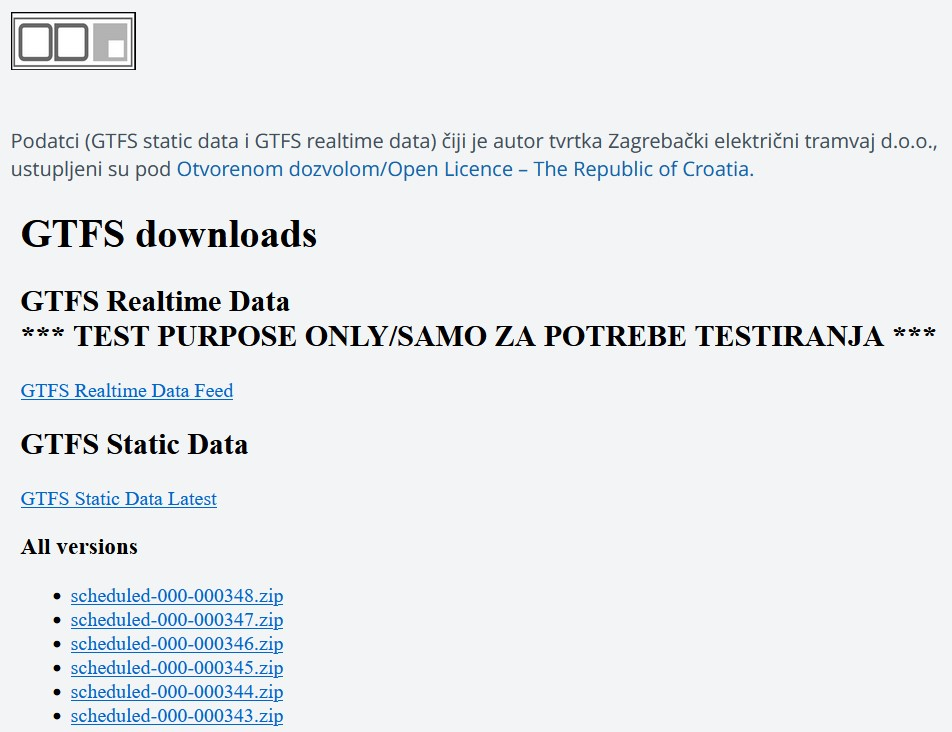
\includegraphics[width=0.7\linewidth]{Figures/zet-stranica.jpg} 
	\caption{ZET stranica za GTFS podatke}
	\label{slk:zet-stranica}
\end{figure} 

\begin{figure}[htb]
	\centering
	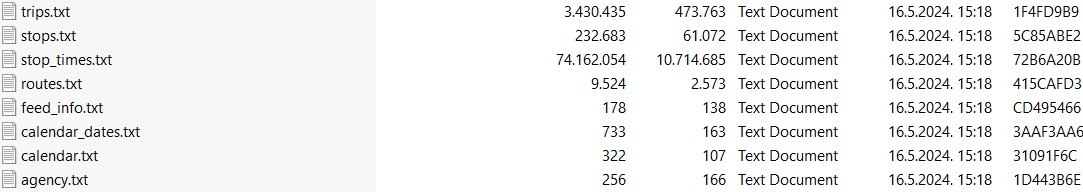
\includegraphics[width=0.7\linewidth]{Figures/zet-podaci.jpg} 
	\caption{ZET GTFS static podaci}
	\label{slk:zet-podaci}
\end{figure} 

Kao što vidimo tu su sve neophodne datoteke (\textit{trips.txt}, \textit{stops.txt}, \textit{stop\_times.txt}, \textit{routes.txt}, \textit{calendar.txt} i \textit{agency.txt}) te par dodatnih datoteka \textit{feed\_info.txt} i \textit{calendar\_dates.txt} koje nisu pretežito korisne za implementaciju aplikacije. Opcionalna datoteka \textit{feed\_info.txt} sadržava opće informacije o GTFS \textit{feed}-u, odnosno  informacije poput naziva agencije koja je stvorila \textit{feed}, vremena kada je \textit{feed} generira, verzije GTFS standarda koja se koristi, i slično.

Pobliže ćemo pogledati datoteke \textit{trips.txt}, \textit{stops.txt}, \textit{stop\_times.txt} i \textit{routes.txt} jer one sadrže temeljne podatke za rad aplikacije.

\subsubsection{trips.txt}

% Please add the following required packages to your document preamble:
% \usepackage[table,xcdraw]{xcolor}
% Beamer presentation requires \usepackage{colortbl} instead of \usepackage[table,xcdraw]{xcolor}
\begin{table}[htb]
	\begin{adjustbox}{width=\columnwidth,center}
	\begin{tabular}{l|l|l|l|l|l|l|l}
		\hline
		\multicolumn{1}{c|}{\textbf{route\_id}} & \multicolumn{1}{c|}{\textbf{service\_id}} & \multicolumn{1}{c|}{\textbf{trip\_id}} & \multicolumn{1}{c|}{\textbf{trip\_headsign}} & \multicolumn{1}{c|}{\textbf{trip\_short\_name}} & \multicolumn{1}{c|}{\textbf{direction\_id}} & \multicolumn{1}{c|}{\textbf{block\_id}} & \multicolumn{1}{c}{\textbf{shape\_id}} \\ \hline
		268 & "0\_21" & "0\_21\_26820\_268\_10001" & "V. Gorica" &  & \textbf{0} & 26820 &  \\ \hline
		8 & "0\_21" & "0\_21\_801\_8\_10002" & "Grač. dolje" & \textbf{} & 1 & 801 &  \\ \hline
		7 & "0\_21" & "0\_21\_701\_7\_10012" & "Arena Zagreb" & \textbf{} & 1 & 701 &  \\ \hline
	\end{tabular}
	\end{adjustbox}
	\caption{Izgled trips.txt}
	\label{tbl:trips}
\end{table}


Bitne informacije u trips.txt su:
\begin{itemize}
	\item \textbf{route\_id} - identifikator rute, odnosno broj linije (npr. Kod 17 Borongaj, to je 17)
	\item \textbf{trip\_id} - identifikator putovanja na pojedinoj ruti (svaka ruta ima više tramvaja koji više puta dnevno putuju na toj ruti)
	\item \textbf{trip\_short\_name} i \textbf{direction\_id} - ime smjera tramvaja i binarni broj koji određuje smjer (npr. Borongaj)
\end{itemize}

Također možemo primijetiti da datoteka sadrži i shape\_id koji se koristi kao ključ za relaciju trips.txt i shapes.txt koja kao što je rečeno sadrži detaljne koordinate putanje pojedine rute, s kojom bi se na karti s lakoćom mogao iscrtati put glatkom neisprekidanom krivuljom.
Ali u ZET-ovim podacima se ne može pronaći shapes.txt te kao obilazak tom problemu uzete su koordinate svih stanica na pojedinoj ruti koje su spojene ravnim linijom. Izgled te linije nije idealan, ali je rješenje približno. Postoje i određene \textit{routing} komponente, ali i takvo rješenje ima svoje nedostatke, ali o tom više u poglavlju o implementaciji klijentske strane aplikacije \ref{sec:frontend}.

\subsubsection{stops.txt}

\begin{table}[htb]
	\begin{adjustbox}{width=\columnwidth,center}
	\begin{tabular}{l|l|l|l|l|l|l|l|l|l}
		\hline
		\multicolumn{1}{c|}{\textbf{stop\_id}} & \multicolumn{1}{c|}{\textbf{stop\_code}} & \multicolumn{1}{c|}{\textbf{stop\_name}} & \multicolumn{1}{c|}{\textbf{stop\_desc}} & \multicolumn{1}{c|}{\textbf{stop\_lat}} & \multicolumn{1}{c|}{\textbf{stop\_lon}} & \multicolumn{1}{c|}{\textbf{zone\_id}} & \multicolumn{1}{c|}{\textbf{stop\_url}} & \textbf{location\_type} & \textbf{parent\_station} \\ \hline
		"98" &  & "Črnomerec" &  & 45.815175 & 15.934464 &  &  & 1 &  \\ \hline
		"100" &  & "Sveti Duh" &  & 45.813468 & 15.942297 &  &  & 1 &  \\ \hline
		"106\_1" & "1" & "Trg J. Jelačića" &  & 45.812906 & 15.977312 &  &  & 0 & 106 \\ \hline
		"106" &  & "Trg J. Jelačića" &  & 45.813038 & 15.976928 &  &  & 1 &  \\ \hline
	\end{tabular}
	\end{adjustbox}
	\caption{Izgled stops.txt}
	\label{tbl:stops}
\end{table}

Bitne informacije u stops.txt su:
\begin{itemize}
	\item \textbf{stop\_id} - identifikator pojedine stanice
	\item \textbf{stop\_name} - naziv stanice
	\item \textbf{stop\_lat} i \textbf{stop\_lon} - koordinate stanice
\end{itemize}


\subsubsection{stop\_times.txt}

\begin{table}[htb]
	\begin{adjustbox}{width=\columnwidth,center}
		\begin{tabular}{l|l|l|l|l|l|l|l|l}
			\hline
			\multicolumn{1}{c|}{\textbf{trip\_id}} & \multicolumn{1}{c|}{\textbf{arrival\_time}} & \multicolumn{1}{c|}{\textbf{departure\_time}} & \multicolumn{1}{c|}{\textbf{stop\_id}} & \multicolumn{1}{c|}{\textbf{stop\_sequence}} & \multicolumn{1}{c|}{\textbf{stop\_headsign}} & \multicolumn{1}{c|}{\textbf{pickup\_type}} & \multicolumn{1}{c|}{\textbf{drop\_off\_type}} & \textbf{shape\_dist\_traveled} \\ \hline
			"0\_21\_26820\_268\_10001" & "00:30:00" & "00:30:00" & "110\_82" & 1 & "V. Gorica" &  &  &  \\ \hline
			"0\_21\_26820\_268\_10001" & "00:32:30" & "00:32:30" & "238\_24" & 2 & "V. Gorica" &  &  &  \\ \hline
			"0\_21\_26820\_268\_10001" & "00:33:40" & "00:33:40" & "450\_24" & 3 & "V. Gorica" &  &  &  \\ \hline
			"0\_21\_26820\_268\_10001" & "00:35:20" & "00:35:20" & "1085\_24" & 4 & "V. Gorica" &  &  &  \\ \hline
		\end{tabular}
	\end{adjustbox}
	\caption{Izgled stop\_times.txt}
	\label{tbl:stop_times}
\end{table}

Bitne informacije u stop\_times.txt su:
\begin{itemize}
	\item \textbf{trip\_id} - identifikator putovanja na pojedinoj ruti
	\item \textbf{arrival\_time} i \textbf{departure\_time} - vrijeme dolaska i odlaska
	\item \textbf{stop\_id} - identifikator pojedine stanice
	\item \textbf{stop\_sequence} - redni broj stanice na putu
\end{itemize}
Ovo je najveća datoteka (oko 70MB, \textasciitilde{}1000000 linija) koja za svako pojedino putovanje (trip\_id) sadrži informacije o svim stanicama na putu, očekivanom vremenu dolaska i odlaska sa stanice i redoslijedu. Ona će biti ključna za iscrtavanje rute i predviđanju lokacije tramvaja.

\subsubsection{routes.txt}

\begin{table}[htb]
	\begin{adjustbox}{width=\columnwidth,center}
	\begin{tabular}{l|l|l|l|l|l|l|l|l}
		\hline
		\multicolumn{1}{c|}{\textbf{route\_id}} & \multicolumn{1}{c|}{\textbf{agency\_id}} & \multicolumn{1}{c|}{\textbf{route\_short\_name}} & \multicolumn{1}{c|}{\textbf{route\_long\_name}} & \multicolumn{1}{c|}{\textbf{route\_desc}} & \multicolumn{1}{c|}{\textbf{route\_type}} & \multicolumn{1}{c|}{\textbf{route\_url}} & \multicolumn{1}{c|}{\textbf{route\_color}} & \textbf{route\_text\_color} \\ \hline
		1 & 0 & "1" & "Zap.kol. - Borongaj" &  & 0 &  & "ffffff" & "000000" \\ \hline
		2 & 0 & "2" & "Črnomerec - Savišće" &  & 0 &  & "ffffff" & "000000" \\ \hline
		3 & 0 & "3" & "Ljubljanica -Savišće" &  & 0 &  & "ffffff" & "000000" \\ \hline
		4 & 0 & "4" & "Savski most - Dubec" &  & 0 &  & "ffffff" & "000000" \\ \hline
	\end{tabular}
	\end{adjustbox}
	\caption{Izgled routes.txt}
	\label{tbl:routes}
\end{table}

Ovdje nam je jedina nova bitna informacija \textbf{route\_long\_name} koja nam daje puno ime rute (početno mjesto i krajnje mjesto)\\
To bi bile najbitnije GTFS static informacije koje su upotrijebljene za izradu aplikacije, koje su od posebne značajnosti za izradu baze podataka koja sprema te odvojene datoteke kao tablice i spaja ih s odgovarajućim ključevima i time omogućuje lako i brzo pretraživanje te formuliranje odgovora \ref{sec:baza}.

\newpage
\subsubsection{ZET realtime podaci}
Na ZET-ovoj stranici se nalazi link za GTFS realtime podatke \ref{slk:zet-stranica} koji kada se skinu su binarna datoteka u .proto formatu. Protobuf je opisan u narednom poglavlju \ref{sec:protobuf}. Ovdje ćemo samo brzo proći kroz konačne podatke kada se obavi deserijalizacija.\\\\
Na slici \ref{slk:reply1} se nalazi jedan mali isječak od inače jako velike poruke (obično sadrže oko 500 - 600 entiteta), ali radi jednostavnosti je prikazan samo jedan.\\\\
Na početku svake poruke se nalazi \textit{header} i možemo primijetiti da se koristi starija verzija GTFS 1.0, sada je aktualna 2.0 verzija koja ima bolje definiranu \textit{schemu} s više informacija i pruža veću fleksibilnost. Također piše da se svaki put šalju svi podaci "FULL\_DATASET" i na kraju je vremenska oznaka generiranja poruke koja je u UNIX formatu.\\\\
Zatim polje \textit{entity} koje sadrži entitet (objekt) koji reprezentira informacije o jednom vozilu. Svaki od njih ima jedinstveni ID i \textit{tripUpdate}. \textit{TripUpdate} se sastoji od osnovnih informacija o putu na kojem je vozilo, ID tog puta, kada je započeo put, je li put prema rasporedu, broj rute kojoj pripada taj put, vremenska oznaka generiranja tih podataka i \textit{stopTimeUpdate} koji sadrži informacije o zadnjoj posjećenoj stanici njen ID, redni broj i vremenska oznaka.\\\\
Jedna stvar koju je vrijedno napomenuti da su ZET-ovi podaci prilično osnovni tjst. sadrže najosnovnije informacije, vjerojatni razlog toga je što su ZET-ovi podaci u fazi razvoja i na stranici je navedeno da je ovo prototip. Na primjer jedna jako velika stvar koja bi bila jako korisna jesu \textit{vehicle} podaci (slika \ref{slk:reply2}) koji sadrže točne geografske lokacije vozila. Trenutačno je aplikacija napravljena tako da na karti prikaže zadnje potvrđene pozicije tramvaja koje su zapravo podaci iz \textit{stopTimeUpdate} odnosno lokacije zadnje posjećenih stanica i markeri koji su predikcije položaja tramvaja temeljene na vremenima iz GTFS static podataka. Implementacija tih vehicle podataka bi izbacilo potrebu za predikcijom i puno olakšala direktno prikazivanje točnih lokacija tramvaja.

\begin{figure}[H]
	\centering
	

	\begin{minipage}[htb]{0.58\linewidth}
		\centering
		
		\begin{lstlisting}[language=Java]
"header": {
	"gtfsRealtimeVersion": "1.0",
	"incrementality": "FULL_DATASET",
	"timestamp": "1702666249"
},
"entity": [
{
	"id": "XNYGO5S0BU",
	"tripUpdate": {
		"trip": {
			"tripId": "0_1_11504_115_10447",
			"startDate": "20231215",
			"scheduleRelationship": "SCHEDULED",
			"routeId": "115"
		},
		"stopTimeUpdate": [
		{
			"stopSequence": 12,
			"arrival": {
				"delay": 145,
				"time": "1702666205"
			},
			"stopId": "1634_22",
			"scheduleRelationship": "SCHEDULED"
		}
		],
		"timestamp": "1702666189"
	}
}
]
		\end{lstlisting} 
		\caption{Dio ZET-ovog GTFS-rt feed-a}
		\label{slk:reply1}
	\end{minipage}
	\hfill
	\begin{minipage}[htb]{0.38\linewidth}
		\centering
		\begin{lstlisting}[language=Java]
			"vehicle": {
				"position": {
					"latitude": 45.8150,
					"longitude": 15.9819,
					"bearing": 120,
					"odometer": 15000.5,
					"speed": 30.5
				}
			}
		\end{lstlisting}
		\caption{Primjer vehicle podataka}
		\label{slk:reply2}
	\end{minipage}
\end{figure}


\newpage
\section[Protobuf]{Protocol buffers}
\label{sec:protobuf}

Protocol Buffers su jezično i platformski neutralni, proširivi mehanizmi za serijalizaciju strukturiranih podataka. Razvijeni od strane Googlea, prvotno su bili namijenjeni internoj uporabi, ali su kasnije postali dostupni pod otvorenom licencom \cite{protobuf}. Glavni cilj protocol buffera je pružiti jednostavnost i visoke performanse, te su posebno dizajnirani kako bi bili manji i brži od XML i JSON formata.


Protobuf koristi .proto datoteke za definiranje strukture podataka koji koriste posebnu sintaksu. Trenutno su podržane verzije proto2 i proto3 u kojima se s ključnom riječi message definira struktura podataka poruke. Na slici \ref{slk:proto} je mali primjer jedne definicije poruke Person koja sadrži tri polja za podatke id, name i email. Svaka od njih mora imati tip podatka i vrijednost koja služi za identifikaciju polja kod binarne serijalizacije. Neki tipovi podataka koji su podržani su int32, int64, float, double, bool, string, enum i ugrađene poruke.

\begin{figure}[H]
	\centering
	\begin{minipage}{0.6\linewidth}
		\begin{lstlisting}[language=Python]
			syntax = "proto3";
			message Person{
				int32 id = 1;
				string name = 2;
				string eamil= 3;
			}
		\end{lstlisting}
	\end{minipage}
	\caption{Primjer .proto definicije}
	\label{slk:proto}
\end{figure}		


Kada smo definirali strukturu svoje poruke potrebno je iskoristiti proto compiler (\textit{protoc}) da bi generirali k\^od koji se koristi za serijalizaciju i deserializaciju podataka u odabranom programskom jeziku (C++, Java, Python, Go, JavaScript i mnogo drugih). Za primjer sa slike \ref{slk:proto} i za programski jezik Python, protoc compiler generira modul person\_pb2 koji sadrži potrebne metode za kreiranje objekata te strukture, serijalizaciju i deserijalizaciju tih podataka. 

\begin{figure}[h]
	\centering
	\begin{minipage}{0.8\linewidth}
		\begin{lstlisting}[language=Python]
			import person_pb2
			
			person = person_pb2.Person()
			person.id = 123
			person.name = "John Doe"
			person.email = "johndoe@example.com"
			
			# Serijalizacija
			serialized_data = person.SerializeToString()
			
			# Deserijalizacija
			new_person = person_pb2.Person()
			new_person.ParseFromString(serialized_data)
		\end{lstlisting}
	\end{minipage}
	\caption{Python k\^od s generiranim proto modulom}
	\label{slk:proto_kod}
\end{figure}

Neke prednosti korištenja protocol buffer-a za razliku od tradicionalnijih opcija poput XML-a i JSON-a su:

\begin{itemize}
	\item Protobuf koristi binarni format za serijalizaciju, koji je mnogo kompaktniji i brži za parsiranje.
	\item Dizajniran s \textit{backward} i \textit{forwards compatibility} na umu 
	\item Međujezična kompatibilnost (\textit{Cross-Language compatibility})
	\item Imaju validaciju schema koji striktno čuvaju strukturu podataka
\end{itemize}

\newpage
\section{Arhitektura sustava}

Sustav se temelji na modelu Klijent-Poslužitelj. Taj model je danas jedan od najčešće korištenih arhitektura za raspodijeljene sustave. On se sastoji od dva dijela, poslužitelja koji nudi uslugu i klijenta koji traži uslugu. Klijent će biti korisnikovo računalo koje pomoću web preglednika koristi klijentski dio aplikacije (React frontend) te putem HTTP komunikacijskog kanala komunicira s poslužiteljskim dijelom aplikacije (node.js i PostgreSQL).\\\\
Klijentski dio aplikacije je izrađen pomoću React.js, popularnog JavaScript okvir za izgradnju korisničkih sučelja, primarno korišten za jednostranične aplikacije (Single-page Application, SPA).\\\\
Poslužiteljski dio aplikacije izrađen je pomoću node.js, koji je također JavaScript okvir, ali za izgradnju server-side aplikacija. Aplikacija će također komunicirati i s relacijskom bazom podataka PostgreSQL. Poslužitelj će obrađivati klijentske zahtjeve i pružati odgovarajuće odgovore nazad.\\

\begin{figure}[htb]
	\centering
	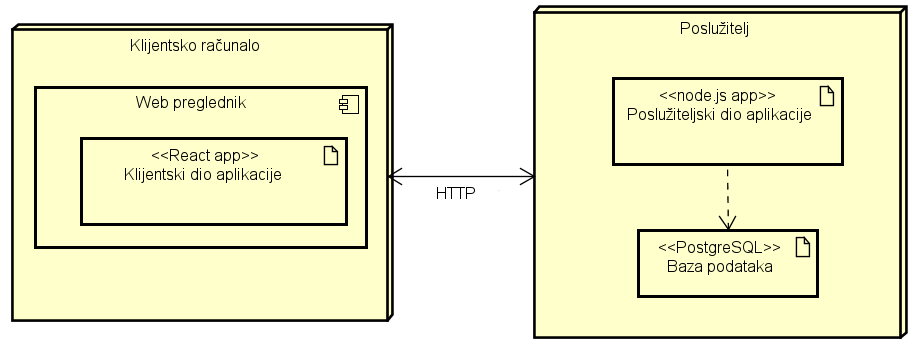
\includegraphics[width=0.8\linewidth]{Figures/arhitektura.png} 
	\caption{Arhitektura sustava}
	\label{slk:sustav}
\end{figure}

\subsection{Baza podataka}
\label{sec:baza}
Baza podataka je izvedena pomoću PostgreSQL-a. PostgreSQL je besplatan i otvoreni, objektno-relacijski sustav za upravljanje bazama podataka. Temelji se na SQL jeziku i nudi brojna proširenja koji olakšavaju pohranu i skaliranje, povećavaju sigurnost te rješavaju probleme paralelnosti pristupa. Nastao je 1986. godine na Kalifornijskom sveučilištu u Berkeleyju. \cite{postgresql}\\

Baza podataka je korištena zbog velike količine podataka iz ZET-ovih statičnih podataka te bi najoptimalniji način upravljanja i pohranom tih podataka bila baza podataka.
Glavne uloge baze podataka u aplikaciji su:
\begin{itemize}
	\item Spremanje ZET-ovih statičnih podataka kao tablice
 	\item Povezivanje tablica statičnih podataka pomoću ključeva u virtualne tablice (\textit{views})
 	\item Funkcije za brzi pronalazak traženih podataka prema nekom parametru
 	\item Formiranje odgovora
\end{itemize}

Ubacivanje podataka iz ZET-ovih datoteka u bazu podataka je automatizirano pomoću python skripte (opisana u narednom poglavlju \ref{sec:skripta}). Datoteke koje smo ubacili su \textit{trips.txt, stops.txt, routes.txt i stop\_times.txt}. One su ubačene kao najobičnije tablice gdje stupce pojedine tablice definira \textit{header} te datoteke (prisjetimo se one su zapravo CSV datoteke! \ref{sec:zet-gtfs}).

Spajanje tih tablica je ostvareno virtualnim tablicama tkzv. pogledi (\textit{views}) koji objedinjuju par tablica u jednu i ostavljaju samo navedene stupce. Sadržaj virtualne tablice dinamički se određuje u trenutku obavljanja operacije nad virtualnom tablicom te se ponovo izvode svaki put kada ih se pozove. Time se izbjegava problem "zastarijevanja" podataka.\\
Neki od pogleda su \textit{stopsjson, tripstops i triptime}.
\textit{Stopsjson} vraća polje \textit{key-value} vrijednosti, gdje je ključ \textit{stop\_id} i vrijednost objekt s imenom i pozicijom stanice. Rezultat vraća kao JSON objekt.
\begin{figure}[h]
	\centering
	\begin{minipage}{0.8\linewidth}
		\begin{lstlisting}[language=SQL]
 		SELECT jsonb_object_agg(stop_id::text, jsonb_build_object('stop_name', stop_name, 'stop_lat', stop_lat, 'stop_lon', stop_lon)) AS stops
		FROM stops;
		\end{lstlisting}
	\end{minipage}
	\caption{K\^od pogleda \textit{stopsjson}}
	\label{slk:stopsjson}
\end{figure}


Pogled \textit{tripstops} spaja tablice \textit{stop\_times} i \textit{stops} pomoću \textit{stop\_id} kao ključa. Objedinjuje informacije tih dviju tablica kako bi imali potpune informacije o putu poput redoslijeda stanica, njihovih naziva i lokacija te vremena dolaska i odlaska.
\begin{figure}[h]
	\centering
	\begin{minipage}{0.8\linewidth}
		\begin{lstlisting}[language=SQL]
 		SELECT  stop_times.trip_id,
				stops.stop_id,
				stop_times.stop_sequence,
				stops.stop_name,
				stops.stop_lat,
				stops.stop_lon,
				stop_times.arrival_time,
				stop_times.departure_time,
				stop_times.stop_headsign
				FROM stop_times
				JOIN stops USING (stop_id)
				ORDER BY stop_times.stop_sequence;
		\end{lstlisting}
	\end{minipage}
	\caption{K\^od pogleda \textit{tripstops}}
	\label{slk:tripstops}
\end{figure}

\begin{figure}[h]
	\centering
	\begin{minipage}{0.8\linewidth}
		\begin{lstlisting}[language=SQL]
			SELECT trip_id, stop_sequence,
			COALESCE(lead(arrival_time) OVER () - arrival_time, '00:00:00'::interval) AS time_till_next_stop
			FROM tripstops
			ORDER BY stop_sequence;
		\end{lstlisting}
	\end{minipage}
	\caption{K\^od pogleda \textit{triptime}}
	\label{slk:triptime}
\end{figure}

\subsection{Pomoćne skripte}
\label{sec:skripta}

\subsection{Backend - node.js}

\subsection{Frontend - REACT}
\label{sec:frontend}

\section{Izgled aplikacije}


%-------------------------------------------------------------------------------
\chapter{Rezultati i rasprava}
\label{pog:rezultati_i_rasprava}


%--- ZAKLJUČAK / CONCLUSION ----------------------------------------------------
\chapter{Zaključak}
\label{pog:zakljucak}


%--- LITERATURA / REFERENCES ---------------------------------------------------

% Literatura se automatski generira iz zadane .bib datoteke / References are automatically generated from the supplied .bib file
% Upiši ime BibTeX datoteke bez .bib nastavka / Enter the name of the BibTeX file without .bib extension

\nocite{*}

\bibliography{literatura}

%--- SAŽETAK / ABSTRACT --------------------------------------------------------

% Sažetak na hrvatskom
\begin{sazetak}
  Unesite sažetak na hrvatskom.

  \blindtext
\end{sazetak}

\begin{kljucnerijeci}
  prva ključna riječ; druga ključna riječ; treća ključna riječ
\end{kljucnerijeci}


% Abstract in English
\begin{abstract}
  Enter the abstract in English.
  
  \blindtext 
\end{abstract}

\begin{keywords}
  the first keyword; the second keyword; the third keyword
\end{keywords}


%--- PRIVITCI / APPENDIX -------------------------------------------------------

% Sva poglavlja koja slijede će biti označena slovom i riječi privitak / All following chapters will be denoted with an appendix and a letter
\backmatter

\chapter{The Code}


\end{document}
